
We tried to find a dataset with handwritten text at the beginning of the project, but it turns out there are not that many available. 
% Not sure what Image is supposed to be referenced here.
The datasets that do exist, like following image example. See Figure {figure: wordsexamples}, they would have needed a lot of preprocessing before we could use them in our project.
We would have had to implement baseline slant normalization, skew correction, skeleton and so on.

Therefore, instead of spending a lot of time preprocessing the datasets, we implemented a Graphic User Interface to create our own dataset.
The biggest advantages of this solution is that our solution records one pixel wide letters and the characters are already separated. 
The most important part of the work, image processing, was thus reduced significantly.



Furthermore, if the vocabulary is relatively large, we found that it became easier for us to test the HMM.
This is because our word training data is made up of randomly chosen samples.

\begin{figure}[h!]
  \centering
  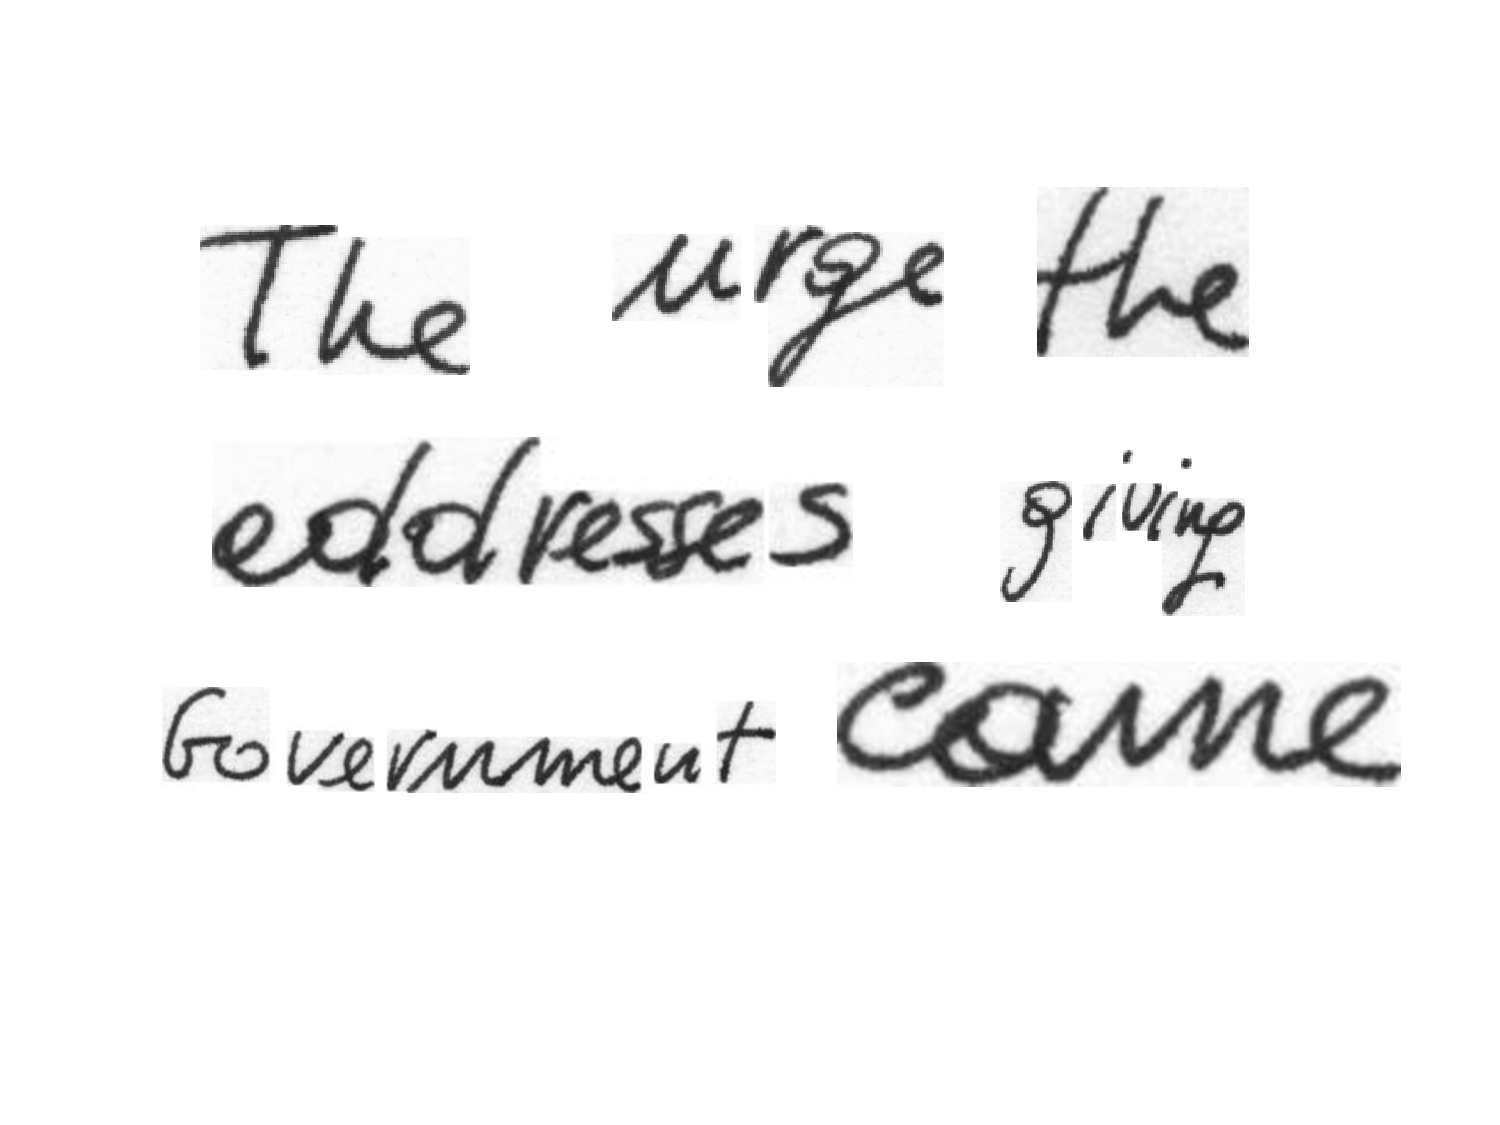
\includegraphics[width=5in]{datasets_examples}
  \caption{Word image examples}
  \label{figure:wordsexamples}
\end{figure}
